\documentclass{article}
\usepackage{graphicx} % Required for inserting images
    \graphicspath{{./Gambar Tugas Besar}{./kode matlab/}}
\usepackage{amsmath} % Buat matriks
\usepackage{amssymb}
\usepackage{pgfplots}
\usepackage{float}
\usepackage{amsmath}
\usepackage[bahasa]{babel}
\usepackage{physics}
\usepackage{hyperref}
\usepackage{tikz}
    \usetikzlibrary{calc,patterns,angles,quotes}
\usepackage{geometry}
\geometry{
 a4paper,
 total={170mm,257mm},
 left=20mm,
 top=20mm,
 }

\usepackage{listings}
\usepackage{minted}
\definecolor{mintedbackground}{rgb}{0.95,0.95,0.95}

\newmintedfile[matlabcode]{matlab}{
bgcolor=mintedbackground,
fontfamily=tt,
linenos=true,
numberblanklines=true,
numbersep=5pt,
gobble=0,
frame=leftline,
framerule=0.4pt,
framesep=2mm,
funcnamehighlighting=true,
tabsize=4,
obeytabs=false,
mathescape=false,
samepage=false, %with this setting you can force the list to appear on the same page
showspaces=false,
showtabs =false,
texcl=false,
}


\renewcommand{\figurename}{Gambar}
\renewcommand{\figureautorefname}{Gambar}
\renewcommand{\lstlistingname}{Kode}

\title{\textbf{Laporan Matematika Sistem: \\
Bandul Matematis}\\
\begin{figure}[h!]
    \centering
    
\includegraphics[width=0.5\linewidth]{logoITS.png}
\end{figure}
}
\author{\textbf{Kelompok 7:}}
\date{}

\begin{document}

\maketitle
\vspace{-1cm}

\begin{enumerate}
    \centering
    \item \textbf{Agustinus Gabriel Situmorang (5002221012)}
    \item \textbf{Teosofi Hidayah Agung (5002221132)}
    \item \textbf{Alief Randiansyah Pradanaputra (5002221172)}
\end{enumerate}

\vspace{0.5cm}
\begin{center}
    \textbf{Dosen Pengampu :\\
        Dr. Didik Khusnul Arif, S.Si, M.Si\\
        (19730930 199702 1 001)}
\end{center}

\vspace{0.5cm}
\begin{center}
    \textbf{Departemen Matematika\\
        Institut Teknologi Sepuluh Nopember\\
        Surabaya}
\end{center}

\newpage

\section{Pendahuluan}
Bandul matematis (atau \textit{simple pendulum}) adalah model fisika yang digunakan untuk menggambarkan gerakan osilasi benda di bawah pengaruh gaya gravitasi, di mana seluruh massa dianggap terpusat pada satu titik (massa titik) yang digantung pada ujung tali atau batang yang tidak bermassa dan tidak elastis. Bandul ini dianggap bergerak tanpa adanya gesekan udara atau hambatan lainnya.
\begin{figure}[h!]
    \centering
    \begin{tikzpicture}[scale=1.5]
        % save length of g-vector and theta to macros
        \pgfmathsetmacro{\Gvec}{1.4}
        \pgfmathsetmacro{\myAngle}{30}
        % calculate lengths of vector components
        \pgfmathsetmacro{\Gcos}{\Gvec*cos(\myAngle)}
        \pgfmathsetmacro{\Gsin}{\Gvec*sin(\myAngle)}

        \draw[brown!70!black,thick] (-2,0) --++ (4,0);
        \fill[pattern = north east lines] (-2,0) rectangle (2,0.2);
        \coordinate (centro) at (0,0);
        \draw[loosely dashed,gray,-] (centro) -- ++ (0,-3.5) node (mary) [black,below]{$ $};
        \draw[thick] (centro) --++ (270+\myAngle:2.8) coordinate (bob) node[midway,above right] {$L$};
        \draw[thick,loosely dashed,black!50] (centro) --++ (270-\myAngle:3) coordinate (bobsd);
        \draw[dashed,red] (bob) arc (270+\myAngle:270-\myAngle:2.8);
        \pic [draw, ->, "$\theta$", angle eccentricity=1.5] {angle = mary--centro--bob};
        \draw [blue,-stealth] (bob) -- ($(bob)!\Gcos cm!(centro)$) node[midway,above right] {$\vb{T}$};
        \draw [-stealth,green!60!black] (bob) -- ($(bob)!-\Gcos cm!(centro)$)
        coordinate (gcos)
            node[midway,above right] {$a\cos\theta$};
        \draw [-stealth,green!60!black] (bob) -- ($(bob)!\Gsin cm!90:(centro)$)
        coordinate (gsin)
            node[midway,above left] {$a\sin\theta$};
        \draw [-stealth] (bob) -- ++(0,-\Gvec)
        coordinate (g)
            node[near end,left] {$g$};
        \pic [draw, ->, "$\theta$", angle eccentricity=1.5] {angle = g--bob--gcos};
        \filldraw [fill=gray!40,draw=black] (bob) circle[radius=0.25] node {$m$};
    \end{tikzpicture}
    \caption{Bandul Matematis}
    \label{fg1}
\end{figure}\\
Bandul matematis memiliki komponen antara lain
\begin{itemize}
    \item Panjang tali ($L$): Panjang tali dianggap tetap dan tidak mengalami peregangan. Ini adalah salah satu parameter penting dalam menentukan periode osilasi.
    \item Massa ($m$): Massa dianggap terkonsentrasi pada satu titik di ujung tali.
    \item Gaya gravitasi ($g$): Bandul bergerak di bawah pengaruh gaya gravitasi yang menarik massa ke bawah.
    \item Sudut deviasi ($\theta$): Sudut antara tali dan garis vertikal pada saat bandul berayun. Jika sudut ini kecil, gerakan bandul dapat dimodelkan sebagai gerak harmonik sederhana (GHS).
\end{itemize}


\section{Asal Usul Persamaan Differensial}

Perumusan persamaan diferensial untuk sistem bandul dapat dijelaskan dengan menggunakan konsep gaya Newton atau torsi. Dalam pembahasan kali ini, akan diturunkan perumusan persamaan diferensial-nya menggunakan konsep gaya Newton, yaitu Hukum Newton II.\\~\\
Bedasarkan Hukum Newton II didapatkan persamaan
\begin{align}
    F=ma \label{1}
\end{align}
dimana $F$ adalah jumlah gaya pada objek, $m$ adalah massa, dan $a$ adalah percepatan. Persamaan Newton dapat diterapkan pada sumbu tangensial saja. Hal ini karena hanya perubahan kecepatan yang menjadi perhatian dan bola dipaksa untuk tetap berada di jalur melingkar. Panah hijau pendek pada \autoref{fg1} mewakili komponen gaya gravitasi pada sumbu tangensial, dan trigonometri dapat digunakan untuk menentukan besarnya. Jadi,
\begin{align}
    F=-mg\sin\theta \label{2}
\end{align}
Dari \eqref{1} dan \eqref{2} didapatkan
\begin{align}
    a=-g\sin\theta \label{3}
\end{align}
Dimana $g$ adalah percepatan gravitasi di dekat permukaan bumi. Tanda negatif di sebelah kanan menunjukkan bahwa sudut $\theta$ dan percepatan $a$ selalu berlawanan arah. Ini masuk akal karena ketika bandul berayun semakin jauh ke kiri, percepatan akan mendorongnya kembali ke arah kanan.\\~\\
Perhatikan bahwa garis putus-putus merah pada \autoref{fg1} menunjukkan lintasan bandul yang dimana membentuk lingkaran dengan pusat pada ujung tali yang menempel pada bidang. Percepatan linier $a$ sepanjang sumbu merah dapat dihubungkan dengan perubahan sudut $\theta$ dengan rumus panjang busur $s$.
\begin{align}
    s & =L\theta                           \\
    v & =L\frac{d\theta}{dt}               \\
    a & =L\frac{d^2\theta}{dt^2} \label{6}
\end{align}
Dari \eqref{3} dan \eqref{6}, didapatkan persamaan
\begin{align}
    L\frac{d^2\theta}{dt^2}=-g\sin\theta
\end{align}
atau dapat ditulis menjadi bentuk persamaan diferensial-nya sebagai berikut
\begin{align}
    \frac{d^2\theta}{dt^2} + \frac{g}{L} \sin \theta = 0
    \label{2.1}
\end{align}
Keterangan: \\
$\theta$: Sudut deviasi dari kesetimbangan (dalam radian) \\
$g$: Percepatan gravitasi \\
$L$: Panjang tali bandul \\

\section{Membentuk \textit{State Space}}
Dari persamaan \eqref{2.1} akan dibentuk dalam \textit{state space}. Untuk membentuk \textit{state space} diperlukan pemisalan yaitu
\begin{equation} \label{eq:x1 x2 theta_defined}
    \begin{aligned}
        x_1 & = \theta,  \\
        x_2 & = \theta'.
    \end{aligned}
\end{equation}
Dengan: \\
$ x_1 = \theta$ adalah sudut deviasi (rad), dan  \\
$x_2 = \theta'$ adalah kecepatan sudut (rad/s) \\
Apabila $x_1$ dan $x_2$ diturunkan terhadap t, maka akan didapat
\begin{align}
    \dot{x_1} & = \theta' = x_2 \label{eq.x1 dot}                                               \\
    \dot{x_2} & = \theta'' = -\frac{g}{L} \sin \theta = -\frac{g}{L} \sin x_1 \label{eq.x2 dot}
\end{align}
Dari persamaan \eqref{eq.x1 dot} dan \eqref{eq.x2 dot} yang didapat adalah persamaan non linear, sebab terdapat $\sin x_1$ yang merupakan salah satu dari fungsi non linear. Sehingga untuk membentuk state space akan dilakukan pelinearan dengan Dari persaman tersebut di dapat bentuk state space sebagai berikut: \\
\[
    \begin{bmatrix}
        \dot{x_1^*} \\
        \dot{x_2^*}
    \end{bmatrix}
    = \begin{bmatrix}
        \dfrac{\partial f_1}{\partial x_1} & \dfrac{\partial f_1}{\partial x_2} \\
        \dfrac{\partial f_2}{\partial x_1} & \dfrac{\partial f_2}{\partial x_2}
    \end{bmatrix} _{\substack{(x_1, x_2)}}
    \begin{bmatrix}
        x_1^* \\
        x_2^*
    \end{bmatrix}
\]
Dengan ($x_1,x_2$) adalah titik kesetimbangan perasamaan. Karena titik kesetimbangan belum diketahui, maka akan dicari titik kesetimbangan sistem yaitu dengan persamaan $\dot{x_1} = 0$ dan $\dot{x_2} = 0$. Sehingga didapat titik kesetimbangan
\begin{align*}
    \dot{x_1} & = 0 \\
    x_2       & = 0
\end{align*}
dan
\begin{align*}
    \dot{x_2}              & = 0                            \\
    -\frac{g}{L} \sin{x_1} & = 0                            \\
    \sin{x_1}              & = 0                            \\
    x_1                    & = n\pi, \quad n \in \mathbb{Z}
\end{align*}
Dengan mengambil salah satu titik kesetimbangan ($x_1,x_2$) adalah ($0,0$). Sehingga akan di dapat \\
\[
    \begin{bmatrix}
        \dot{x_1^*} \\
        \dot{x_2^*}
    \end{bmatrix}
    = \begin{bmatrix}
        0                      & 1 \\
        -\dfrac{g}{L} \cos x_1 & 0
    \end{bmatrix} _{\substack{(0, 0)}}
    \begin{bmatrix}
        x_1^* \\
        x_2^*
    \end{bmatrix}
\]
\[
    \begin{bmatrix}
        \dot{x_1^*} \\
        \dot{x_2^*}
    \end{bmatrix}
    = \begin{bmatrix}
        0                    & 1 \\
        -\dfrac{g}{L} \cos 0 & 0
    \end{bmatrix} _{\substack{(0, 0)}}
    \begin{bmatrix}
        x_1^* \\
        x_2^*
    \end{bmatrix}
\]
\[
    \begin{bmatrix}
        \dot{x_1^*} \\
        \dot{x_2^*}
    \end{bmatrix}
    = \begin{bmatrix}
        0             & 1 \\
        -\dfrac{g}{L} & 0
    \end{bmatrix} _{\substack{(0, 0)}}
    \begin{bmatrix}
        x_1^* \\
        x_2^*
    \end{bmatrix}
\]
Maka bentuk state space persamaan diferensial di atas adalah
\begin{equation}
    \begin{bmatrix}
        \dot{x_1} \\
        \dot{x_2}
    \end{bmatrix}
    = \begin{bmatrix}
        0             & 1 \\
        -\dfrac{g}{L} & 0
    \end{bmatrix}
    \begin{bmatrix}
        x_1 \\
        x_2
    \end{bmatrix} \label{eq.state space A aja}
\end{equation}

\section{Nilai Eigen}
Berdasarkan persmaaan \textit{state space} \eqref{eq.state space A aja}, dengan matriks $A$ adalah
$
    \begin{bmatrix}
        0             & 1 \\
        -\dfrac{g}{L} & 0
    \end{bmatrix}
$
Maka nilai eigen sistem dapat dicari dengan persamaan
\begin{align*}
    |A- \lambda I| = 0                 \\
    \left| \begin{array}{cc}
               -\lambda     & 1        \\
               -\frac{g}{L} & -\lambda
           \end{array} \right| = 0 \\
    {\lambda}^2 - (-\frac{g}{L}) = 0   \\
    {\lambda}^2 +\frac{g}{L} = 0       \\
    \left(\lambda - \sqrt{\frac{g}{L}}i\right)\left(\lambda + \sqrt{\frac{g}{L}}i\right) = 0
\end{align*}
Maka di dapat nilai eigen yaitu  ${\lambda}_1 = \sqrt{\frac{g}{L}}i$ dan ${\lambda}_2 = -\sqrt{\frac{g}{L}}i$.

\section{Vektor Eigen}
Vektor eigen dapat dicari dengan persamaan \[
    (A - \lambda I) \mathbf{v} = 0
\]
dengan mengambil ${\lambda}_1 = \sqrt{\frac{g}{L}}i$ akan di dapat
\[
    \begin{bmatrix}
        -\sqrt{\frac{g}{L}}i & 1                    \\
        -\frac{g}{L}         & -\sqrt{\frac{g}{L}}i
    \end{bmatrix}
    \begin{bmatrix}
        x \\
        y
    \end{bmatrix}
    = \begin{bmatrix}
        0 \\
        0
    \end{bmatrix}
\]
Dengan melakukan OBE $(-\sqrt{\frac{g}{L}}i)B_1 + B_2$ di dapat
\[
    \begin{bmatrix}
        -\sqrt{\frac{g}{L}}i & 1 \\
        0                    & 0
    \end{bmatrix}
    \begin{bmatrix}
        x \\
        y
    \end{bmatrix}
    = \begin{bmatrix}
        0 \\
        0
    \end{bmatrix}
\]

\[ (-\sqrt{\frac{g}{L}}i)x + y = 0
\]
\[
    y = (\sqrt{\frac{g}{L}}i)x
\]
misal $x=t$ maka akan di dapat $y =(\sqrt{\frac{g}{L}}i)t $. Sehingga di dapat vektor eigen
\[
    V = \begin{bmatrix}
        1 \\
        \sqrt{\frac{g}{L}}i
    \end{bmatrix}
\]

\section{{Penyelesaian Umum Persamaan Differensial}}
Penyelesaian umum persamaan diferensial adalah menggunakan persamaan berikut
\[
    \begin{bmatrix}
        x_1 \\
        x_2
    \end{bmatrix}
    = C_1e^{{\lambda}_1t}v_1 + C_2e^{{\lambda}_2t}v_2
\]
Karena nilai eigen yang didapat adalah imajiner maka akan dicari $v_1$ dan $v_2$ dari 1 vektor eigen yang didapat sebelumnya yaitu dengan memisahkan $v_1$ adalah bagian real dan $v_2$ adalah bagian imajiner.
\[
    T= e^{{\lambda}_1t}v \\
\]
\[
    T= e^{\sqrt{\frac{g}{L}}it} \begin{bmatrix}
        1 \\
        \sqrt{\frac{g}{L}}i
    \end{bmatrix}
\]
\[
    T= \begin{bmatrix}
        \cos\left({\sqrt{\frac{g}{L}} t}\right) + i \sin\left({\sqrt{\frac{g}{L}} t}\right)
    \end{bmatrix}
    \begin{bmatrix}
        1 \\
        \sqrt{\frac{g}{L}} i
    \end{bmatrix}
\]
\[
    T= \begin{bmatrix}
        \cos\left({\sqrt{\frac{g}{L}} t}\right) + i \sin\left({\sqrt{\frac{g}{L}} t}\right) \\
        -\sqrt{\frac{g}{L}} \sin\left({\sqrt{\frac{g}{L}} t}\right) + i \sqrt{\frac{g}{L}} \cos\left({\sqrt{\frac{g}{L}} t}\right)
    \end{bmatrix}
\]
maka didapat
\[
    v_1= \begin{bmatrix}
        \cos\left({\sqrt{\frac{g}{L}} t}\right) \\
        -\sqrt{\frac{g}{L}} \sin\left({\sqrt{\frac{g}{L}} t}\right)
    \end{bmatrix} \quad v_2 = \begin{bmatrix}
        \sin\left({\sqrt{\frac{g}{L}} t}\right) \\
        \sqrt{\frac{g}{L}} \cos\left({\sqrt{\frac{g}{L}} t}\right)
    \end{bmatrix}
\]
Sehingga di dapat PUPD:
\[
    \begin{bmatrix}
        x_1 \\
        x_2
    \end{bmatrix}
    = C_1e^{{\lambda}_1t}v_1 + C_2e^{{\lambda}_2t}v_2
\]
\[
    \begin{bmatrix}
        x_1 \\
        x_2
    \end{bmatrix}
    = C_1\begin{bmatrix}
        \cos\left({\sqrt{\frac{g}{L}} t}\right) \\
        -\sqrt{\frac{g}{L}} \sin\left({\sqrt{\frac{g}{L}} t}\right)
    \end{bmatrix}  + C_2 \begin{bmatrix}
        \sin\left({\sqrt{\frac{g}{L}} t}\right) \\
        \sqrt{\frac{g}{L}} \cos\left({\sqrt{\frac{g}{L}} t}\right)
    \end{bmatrix}
\]

Pada bab berikutnya akan digunakan penyelesaian standar dengan mensubtitusi $C_1=1$ dan $C_2=0$. Tidak lupa kita asumsikan nilai gaya gravitasi bumi $g=9.8$ dan panjang lengan bandul $L=1$.

\section{Kestabilan}
Berdasarkan nilai eigen yang didapat sebelumnya, terlihat bahwa nilai eigennya adalah imanjiner murni sehingga persamaan differensial stabil tetapi bukan asimtotis dengan bentuk senter. Selanjutnya akan dilakukan simulasi untuk melihat bagaimana kestabilan sistem terhadap grafik penyelesaian sistem. Berikut diberikan grafik penyelesaian $x_1$ dan $x_2$.
\begin{figure}[h!]
    \centering
    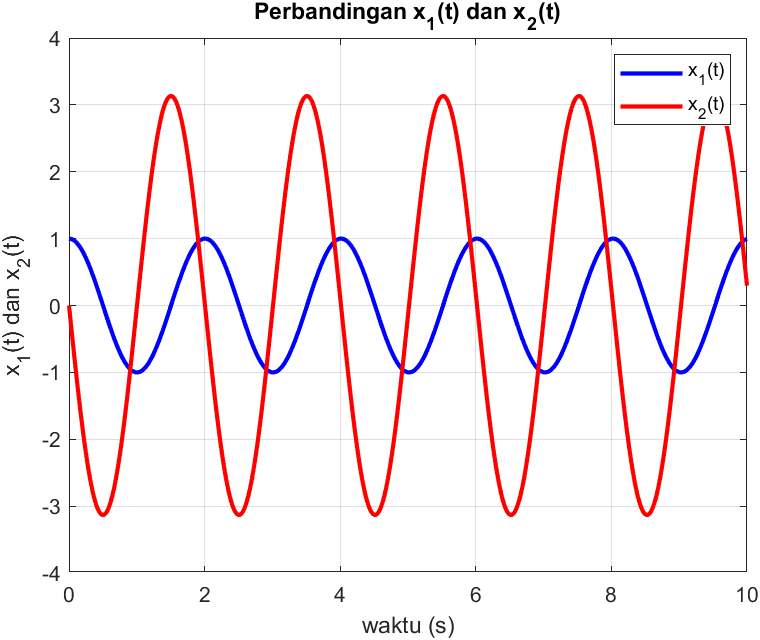
\includegraphics[scale=0.7]{Gambar Tugas Besar/Grafik PUPD.png}
    \caption{Grafik $x_1(t)$ dan $x_2(t)$}
\end{figure}

Dari informasi \eqref{eq:x1 x2 theta_defined}, telah didefinisikan bahwa $x_1$ dan $x_2$ adalah nilai dalam radian (1 radian $\approx 57,2958^\circ$). Kemudian dapat kita notasikan besarnya sudut $x_1=\theta$ dan kecepatan sudut dalam radian per detik $x_2=\omega$, sesuai yang telah dipelajari di fisika. Ilustrasi gerakan bandul saat waktu $t$ adalah sebagai berikut:
\begin{figure}[H]
    \centering
    \begin{tikzpicture}
        % Support
        \fill (-1.5,0) rectangle(1.5,0.1);
        \node[draw, rectangle, fill=brown!10, text width=1.5cm, align=left] at (0, 1) {
            $\theta=57^\circ$

            $\omega=0$

            $t=0$
        };
        % Bob's trajectory
        \draw[dashed] (-60:4) arc(-60:-120:4);

        % Rod + Bob
        \draw (0,0) coordinate (O) -- (-60:4) node[fill,circle](m){};
        \draw (m) ++ (-60:0.3) node[](mshift){};
        % Weight Force
        \draw[-latex,red,thick] (mshift) node[below]{$\omega$};

        %garis pembatas
        \draw[green,dashed] (0,0) -- (-90:4);

        % Light gray pendulum
        \draw[black!10] (0,0) -- (-90:4) node[fill,circle](t0){};
        \draw[black!10] (0,0) -- (-120:4) node[fill,circle]{};

        % Angle indicator using pic
        \pic [draw, ->, "$\theta$", angle eccentricity=1.5, angle radius=0.5cm,blue] {angle = t0--O--m};

        \draw[black, very thick] (-3,-5) rectangle (3,2);
    \end{tikzpicture}
    \begin{tikzpicture}
        % Support
        \fill (-1.5,0) rectangle(1.5,0.1);
        \node[draw, rectangle, fill=brown!10, text width=1.5cm, align=left] at (0, 1) {
            $\theta=0^\circ$

            $\omega=-3$

            $t=0.5$
        };
        % Bob's trajectory
        \draw[dashed] (-60:4) arc(-60:-120:4);

        % Rod + Bob
        \draw (0,0) coordinate (O) -- (-90:4) node[fill,circle](m){};
        \draw (m) ++ (-60:0.3) node[](mshift){};
        % Weight Force
        \draw[-latex,red,thick] (mshift) arc(-80:-110:2.5) node[below left]{$\omega$};

        %garis pembatas
        \draw[green,dashed] (0,0) -- (-90:4);

        % Light gray pendulum
        \draw[black!10] (0,0) -- (-60:4) node[fill,circle](t0){};
        \draw[black!10] (0,0) -- (-120:4) node[fill,circle]{};

        % Angle indicator using pic
        \pic [draw, "$\theta$", angle eccentricity=1.5, angle radius=0cm,blue,right] {angle = m--O--m};

        \draw[black, very thick] (-3,-5) rectangle (3,2);
    \end{tikzpicture}\\

    \begin{tikzpicture}
        % Support
        \fill (-1.5,0) rectangle(1.5,0.1);
        \node[draw, rectangle, fill=brown!10, text width=1.5cm, align=left] at (0, 1) {
            $\theta=-57^\circ$

            $\omega=0$

            $t=1$
        };
        % Bob's trajectory
        \draw[dashed] (-60:4) arc(-60:-120:4);

        % Rod + Bob
        \draw (0,0) coordinate (O) -- (-120:4) node[fill,circle](m){};
        \draw (m) ++ (-60:0.3) node[](mshift){};
        % Weight Force
        \draw[-latex,red,thick] (mshift) node[below left]{$\omega$};

        %garis pembatas
        \draw[green,dashed] (0,0) -- (-90:4);

        % Light gray pendulum
        \draw[black!10] (0,0) -- (-90:4) node[fill,circle](t0){};
        \draw[black!10] (0,0) -- (-60:4) node[fill,circle]{};

        % Angle indicator using pic
        \pic [draw, ->, "$\theta$", angle eccentricity=1.5, angle radius=0.5cm,blue]
        {angle = m--O--t0};

        \draw[black, very thick] (-3,-5) rectangle (3,2);
    \end{tikzpicture}
    \begin{tikzpicture}
        % Support
        \fill (-1.5,0) rectangle(1.5,0.1);
        \node[draw, rectangle, fill=brown!10, text width=1.5cm, align=left] at (0, 1) {
            $\theta=0^\circ$

            $\omega=3$

            $t=1.5$
        };
        % Bob's trajectory
        \draw[dashed] (-60:4) arc(-60:-120:4);

        % Rod + Bob
        \draw (0,0) coordinate (O) -- (-90:4) node[fill,circle](m){};
        \draw (m) ++ (-60:0.3) node[](mshift){};
        % Weight Force
        \draw[-latex,red,thick] (mshift) arc(-90:-60:2.5) node[below right]{$\omega$};

        %garis pembatas
        \draw[green,dashed] (0,0) -- (-90:4);

        % Light gray pendulum
        \draw[black!10] (0,0) -- (-60:4) node[fill,circle](t0){};
        \draw[black!10] (0,0) -- (-120:4) node[fill,circle]{};

        % Angle indicator using pic
        \pic [draw, "$\theta$", angle eccentricity=1.5, angle radius=0cm,blue,left]
        {angle = m--O--m};
        \draw[black, very thick] (-3,-5) rectangle (3,2);
    \end{tikzpicture}
    \caption{Ilustrasi gerakan bandul pada detik ke-$t$}
\end{figure}
Dari ilustrasi diatas, diperoleh informasi bahwa kecepatan sudut bernilai negatif saat bandul bergerak searah jarum jam dan sebaliknya positif ketika bergerak berlawanan arah jarum jam. Selain itu, kecepatan sudut bandul akan nol ketika berada pada ujung periodik, sedangkan bernilai maksimal ketika berada pada posisi yang tegak lurus terhadap bidang gantung.

\section{Kekontrolan}
Berdasarkan persamaan \eqref{eq.state space A aja} didapat bentuk \textit{state space} dalam bentuk $\dot{x} = Ax + Bu$ dengan B bernilai 0, sehingga sistem tidak dapat dikontrol. Akan tetapi akan dibuat asumsi jika persamaan diberikan input kontrol pada sistem, sehingga persamaan menjadi:

\begin{align}
    \frac{d^2\theta}{dt^2} = -\frac{g}{L} \sin \theta + u \label{eq.input kontrol}
\end{align}
Sehingga persamaan state space menjadi: \\
\begin{equation}
    \begin{bmatrix} \dot{x}_1 \\ \dot{x}_2 \end{bmatrix} =
    \begin{bmatrix} 0 & 1 \\ -\frac{g}{L} & 0 \end{bmatrix}
    \begin{bmatrix} x_1 \\ x_2 \end{bmatrix} +
    \begin{bmatrix} 0 \\ 1 \end{bmatrix} u \label{eq.statespace dengan kontrol}
\end{equation}
Dengan begitu matriks B sudah diketahui dan dapat dianalisis kekontrolannya.
Dengan menggunakan Teorema Matriks Kekontrolan: $M_c = ( B \,|\, AB \,|\, ... \,|\,A^{n-1}B)$, sistem dikatakan terkontrol apabila $rank(M_c)=n$, dengan n adalah banyaknya variabel sistem. Maka akan dicek kekontrolan persamaan \eqref{eq.statespace dengan kontrol} dengan matriks $M_c$.
\begin{align*}
    B                   & = \begin{bmatrix} 0 \\ 1 \end{bmatrix} \\
    AB = \begin{bmatrix}
             0             & 1 \\
             -\dfrac{g}{L} & 0
         \end{bmatrix}
    \begin{bmatrix}
        0 \\ 1
    \end{bmatrix} & = \begin{bmatrix}
                          1 \\
                          0 \\
                      \end{bmatrix}
\end{align*}
Sehingga matriks $M_c = ( B\,|\,AB )$ adalah
\[
    M_c = \begin{bmatrix}
        0 & 1 \\
        1 & 0
    \end{bmatrix} \\
\]
Dan jika dilihat, rank dari matriks $rank(M_c) = 2$. Sehingga karena $rank(M_c) = 2 = n$ maka sistem terkontrol.

\section{Keteramatan}
Berdasarkan persamaan \eqref{eq.statespace dengan kontrol}, jika variabel yang dapat diamati berupa $x_1$ atau sudut deviasinya, maka bentuknya outputnya adalah
\[
    y =
    \begin{bmatrix}
        1 & 0 \
    \end{bmatrix}
    \begin{bmatrix}
        x_1 \\ x_2
    \end{bmatrix}
\]
Dari persamaan ini diketahui jika $C = \begin{bmatrix}
        1 & 0
    \end{bmatrix}$. Maka akan di analisis keteramatan dari sistem, yaitu dengan menggunakan teorema, jika matriks keteramatan memliki rank sama dengan n. Dengan matriks keteramatan adalah
\[
    M_o = \begin{bmatrix}
        C \\ -- \\ CA \\ -- \\ CA^2 \\ -- \\ ... \\ -- \\ CA^{n-1}
    \end{bmatrix}
\]
Dengan begitu dapat dihitung $C$ dan $CA$ yaitu
\begin{align*}
    C  & = \begin{bmatrix} 1 & 0 \end{bmatrix} \\ \\
    CA & = \begin{bmatrix}
               1 & 0
           \end{bmatrix}
    \begin{bmatrix}
        0            & 1 \\
        -\frac{g}{L} & 0
    \end{bmatrix}                       \\
    CA & = \begin{bmatrix}
               0 & 1
           \end{bmatrix}
\end{align*}
Sehingga matriks keteramatan yaitu
\[
    M_o = \begin{bmatrix}
        1 & 0 \\
        0 & 1
    \end{bmatrix}
\]
Dan jika dilihat, rank dari matriks $rank(M_o) = 2$. Sehingga karena $rank(M_o) = 2 = n$ maka sistem teramati.

\section{Interpretasi}
\indent Setelah dilakukan perhitungan dari awal hingga menghasilkan penyelesaian umum sistem persamaan differensial dan sifat-sifat sistem, dapat di ambil interpretasinya yaitu
\begin{enumerate}
    \item Berdasarkan penyelesaian umum yang didapat sebelumnya, baik $x_1$ sebagai sudut deviasi dan $x_2$ sebagai kecepatan sudut, keduanya begantung pada grafik $\cos$ dan $\sin$, hal ini berakibat bandul akan berosilasi atau bergerak bolak balik.

    \item Berdasarkan analisis kestabilan yang telah dilakukan sebelumnya, nilai eigen dari sistem adalah imajiner murni dengan bagian real imajinernya adalah $0$ maka bandul bergerak secara stabil dan konstan,  artinya bandul tidak pernah berhenti atau kehilangan energi.

    \item Berdasarkan analisis kekontrolan yang telah dilakukan, sistem adalah sistem yang terkontrol. Artinya, apabila sistem diberikan input kontol, maka sistem dapat didesain menjadi sistem yang stabil atau menjadi lebih cepat menuju titik kesetimbangan dengan desain input kontrol tertentu.

    \item Berdasarkan analisi keteramatan yang telah dilakukan, sistem adalah sistem yang teramati. Artinya, melalui varibal yang dapat diamati pada suatu output, dapat dibuat suatu observer yang dapat mengamati semua variabel, walaupun salah satu variabel tidak dapat diamati.

\end{enumerate}

\section{Desain Kontrol}
Pada analisis kestabilan yang dilakukan, terlihat jika sistem stabil tetapi tidak stabil asimtotis. Hal ini disebabkan karena nilai eigen yang didapat adalah imajiner murni. Sehingga sistem akan di desain kontrol dengan kendali umpan balik \textit{closed loop}. Dengan input yang diberikan adalah $u = -Fx(t)$ dengan nilai eigen tujuan adalah conjugate kompleks dengan bagian real $\lambda_{1,2} < 0$. Dengan input $u = -Fx(t)$ maka persamaan state space
\[ \dot{x} = Ax(t) + Bu \\ \]
\[ \dot{x} = Ax(t) - BFx(t) \\ \]
\[ \dot{x} = (A - BF)x(t) \]
Untuk mencari matriks $F$ diperlukan bentuk matriks $F$ yang sesuai. Seperti yang diketahui, jika matriks dari $\dot{x}$ adalah matriks $2 \times 1$, dengan perkalian matriks $A$ dengan $x$ adalah matriks $2 \times 1$, dan matriks $B$ adalah matriks $2 \times 1$, maka agar matriks $\dot{x}$ tetap dalam bentuk matriks $2 \times 1$, matriks $F$ haruslah berukuran $1 \times 2$. Dengan pemisalan $F = [k_1 \quad k_2]$, maka


\[
    A - BF =
    \begin{bmatrix}
        0            & 1 \\
        -\frac{g}{L} & 0
    \end{bmatrix} - \begin{bmatrix}
        0 \\ 1
    \end{bmatrix}
    \begin{bmatrix}
        k_1 & k_2
    \end{bmatrix}
\]
\[A - BF =
    \begin{bmatrix}
        0            & 1 \\
        -\frac{g}{L} & 0
    \end{bmatrix} - \begin{bmatrix}
        0   & 0   \\
        k_1 & k_2
    \end{bmatrix}
\]
\[ A - BF=
    \begin{bmatrix}
        0                  & 1    \\
        -\frac{g}{L} - k_1 & -k_2
    \end{bmatrix}
\]
Selanjutnya, nilai $k_1$ dan $k_2$ akan dihitung menggunakan MATLAB dengan asumsi nilai:
\begin{itemize}
    \item $g = 9.81 \, \text{m/s}^2$
    \item $L = 1 \, \text{m}$
\end{itemize}
Dan nilai eigen tujuan adalah ${\lambda}_{1,2}= -1 \pm i$, akan didapat nilai $F = \begin{bmatrix}
        -7.81 & 2
    \end{bmatrix}$.
Hal ini berakibat menghasilkan sistem dengan kontrol yaitu
\[
    \begin{bmatrix} \dot{x}_1 \\ \dot{x}_2 \end{bmatrix} =
    \begin{bmatrix} 0 & 1 \\ -\frac{g}{L} & 0 \end{bmatrix}
    \begin{bmatrix} x_1 \\ x_2 \end{bmatrix} +
    \begin{bmatrix} 0 \\ 1 \end{bmatrix} u
\]
\[
    \begin{bmatrix} \dot{x}_1 \\ \dot{x}_2 \end{bmatrix} =
    \left(
    \begin{bmatrix} 0 & 1 \\ -\frac{g}{L} & 0 \end{bmatrix}
    -
    \begin{bmatrix} 0 \\ 1 \end{bmatrix}
    \begin{bmatrix} -7.81 & 2 \end{bmatrix}
    \right)
    \begin{bmatrix} x_1 \\ x_2 \end{bmatrix}
\]
\begin{equation}
    \begin{bmatrix} \dot{x}_1 \\ \dot{x}_2 \end{bmatrix} =
    \begin{bmatrix} 0 & 1 \\ -\frac{g}{L} + 7.81 & -2 \end{bmatrix}
    \begin{bmatrix} x_1 \\ x_2 \end{bmatrix} \label{eq. sistem kontrol}
\end{equation}

\section{Simulasi Desain Kontrol}
Simulasi dilakukan membandingkan sistem sebelum dikontrol \eqref{eq.state space A aja} dengan setelah diberikan input kontrol \eqref{eq. sistem kontrol}
\begin{figure}[H]
    \centering
    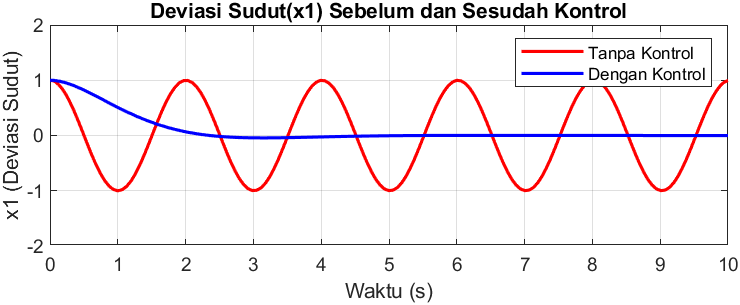
\includegraphics[width=0.6\linewidth]{Gambar Tugas Besar/x1 Kekontrolan.png}
    \caption{Perbandingan $x_1$ Sebelum dan Sesudah Kontrol}
    \label{fig:simulasi2}
\end{figure}
\begin{figure}[H]
    \centering
    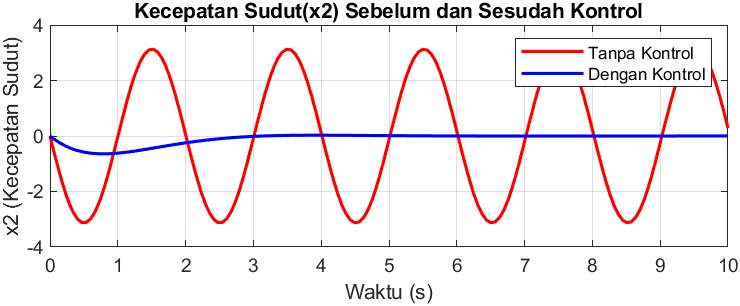
\includegraphics[width=0.6\linewidth]{Gambar Tugas Besar/x2 Kekontrolan.png}
    \caption{Perbandingan $x_2$ Sebelum dan Sesudah Kontrol}
    \label{fig:simulasi1}
\end{figure}
Perubahan yang cukup signifikan pada grafik diatas terjadi karena pergerakan bandul yang telah dipengaruhi faktor eksternal seperti contohnya gaya gesek kinetik. Bandul akan kehilangan gaya osilasinya dan suatu saat akan di posisi diam.


\section{Desain Observer}
Berdasarkan analisis sifat sistem pada bagian Keteramatan, dapat dilihat bahwa sistem \eqref{eq. sistem kontrol} teramati. Maka akan didesain observer dengan
\begin{equation*}
    A = \begin{bmatrix} 0 & 1 \\ -\frac{g}{L} & 0 \end{bmatrix} \\
    \quad C= \begin{bmatrix}
        1 & 0
    \end{bmatrix}
\end{equation*}
yang akan dikontruksi matriks K sedemikian sehingga nilai eigen $A-KC$ bernilai $-1 \pm i$.
Polinomial karakteristik $(A-KC)$ yang diinginkan yaitu
\[ w(\lambda) = (\lambda+1+i)(\lambda+1-i) \]
\[w(\lambda) = {\lambda}^2+2\lambda+2\]
Karena $C_{1 \times 2}$ maka $K_{2 \times 1} = \begin{bmatrix}
        k_1 \\ k_2
    \end{bmatrix}$ dan
\begin{align*}
    A-KC & =
    \begin{bmatrix}
        0 & 1 \\ -\frac{g}{L} & 0
    \end{bmatrix} -
    \begin{bmatrix}
        k_1 \\ k_2
    \end{bmatrix}
    \begin{bmatrix}
        1 & 0
    \end{bmatrix}                             \\
         & = \begin{bmatrix}
                 0 & 1 \\ -\frac{g}{L} & 0
             \end{bmatrix} -
    \begin{bmatrix}
        k_1 & 0 \\ k_2 & 0
    \end{bmatrix}                          \\
         & = \begin{bmatrix}
                 -k_1 & 1 \\ -\frac{g}{L} - k_2 & 0
             \end{bmatrix}
\end{align*}
Dengan menggubakan Matlab akan dicari nilai k sesuai dengan nilai eigen $A-KC$ yang diinginkan dengan asumsi nilai:
\begin{itemize}
    \item $g = 9.81 \, \text{m/s}^2$
    \item $L = 1 \, \text{m}$
\end{itemize}
Akan didapat nilai $K = \begin{bmatrix}
        2 \\ 0.7961
    \end{bmatrix}$. Sehingga Observer sistem adalah
\begin{align*}
    \dot{\hat{x}} & = Ax(t) + Bu(t) + K(y(t)-\hat{y}(t))
\end{align*}
\begin{equation}
    \dot{\hat{x}} = Ax(t) + Bu(t) + K(y(t)-C\hat{x}(t)) \label{eq. desain observer}
\end{equation}
Dengan
\begin{align*}
    A     & = \begin{bmatrix} 0 & 1 \\ -\frac{g}{L} & 0 \end{bmatrix}
    \quad & B                                                         & = \begin{bmatrix}
                                                                              0 \\ 1
                                                                          \end{bmatrix} \\
    C     & = \begin{bmatrix}
                  1 & 0
              \end{bmatrix}
    \quad & K                                                         & = \begin{bmatrix}
                                                                              2 \\ 0.7961
                                                                          \end{bmatrix}
\end{align*}


\section{Simulasi Desain Observer}
Berdasarkan persamaan \eqref{eq. desain observer}, akan dilakukan simulasi dengan membandingkan setiap variabel tanpa kontrol dan adanya kontrol dengan observernya.
\begin{figure}[H]
    \centering
    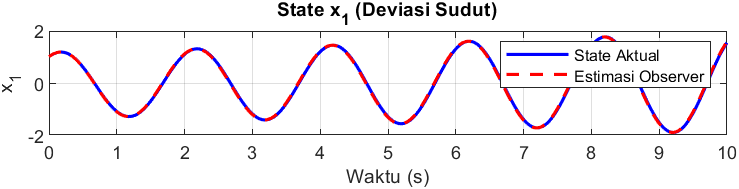
\includegraphics[width=\linewidth]{Gambar Tugas Besar/x1 Observer tanpa kontrol.png}
    \caption{Perbandingan $x_1$ Tanpa Kontrol Sebelum dan Sesudah Desain Observer }
    \label{fig:simulasi}
\end{figure}

\begin{figure}[H]
    \centering
    \includegraphics[width=\linewidth]{Gambar Tugas Besar/X2 Observer tanpa kontrol.png}
    \caption{Perbandingan $x_2$ Tanpa Kontrol Sebelum dan Sesudah Desain Observer}
    \label{fig:simulasi}
\end{figure}

\begin{figure}[H]
    \centering
    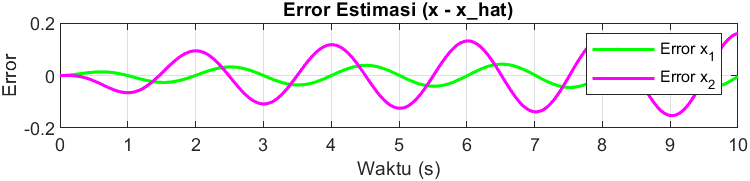
\includegraphics[width=\linewidth]{Gambar Tugas Besar/error x-x topi tanpa kontrol.png}
    \caption{Perbandingan Error $x - \hat{x}$ Tanpa Kontrol }
    \label{fig:simulasi}
\end{figure}

%yg dengan kontrol

\begin{figure}[H]
    \centering
    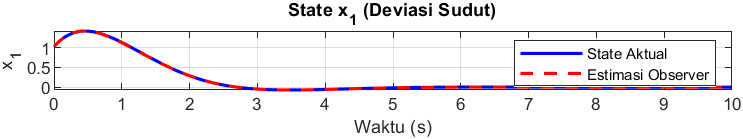
\includegraphics[width=\linewidth]{Gambar Tugas Besar/X1 Observer dengan kontrol.png}
    \caption{Perbandingan $x_1$ Dengan Kontrol Sebelum dan Sesudah Desain Observer }
    \label{fig:simulasi}
\end{figure}

\begin{figure}[H]
    \centering
    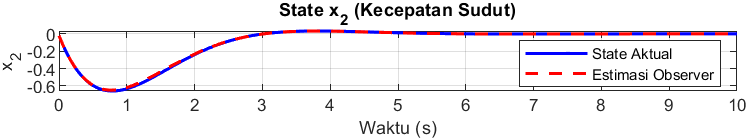
\includegraphics[width=\linewidth]{Gambar Tugas Besar/X2 Observer dengan kontrol.png}
    \caption{Perbandingan $x_2$ Dengan Kontrol Sebelum dan Sesudah Desain Observer}
    \label{fig:simulasi}
\end{figure}

\begin{figure}[H]
    \centering
    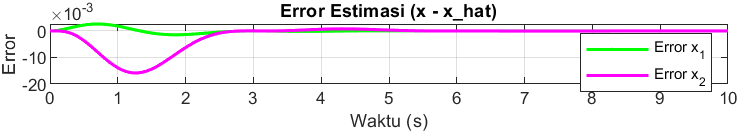
\includegraphics[width=\linewidth]{Gambar Tugas Besar/error x-x topi dengan kontrol.png}
    \caption{Perbandingan Error $x - \hat{x}$ Dengan Kontrol }
    \label{fig:simulasi}
\end{figure}

\section{\textit{Root Mean Square Error} (RMSE)}
\textit{Root Mean Square Error} (RMSE) adalah metrik yang sering digunakan untuk mengukur perbedaan antara nilai yang diprediksi atau diobservasi dengan nilai aktual. Dalam konteks perbandingan dengan nilai error sistem aktual dan sistem observer, rumus RMSE dinyatakan sebgai:

\begin{align*}
    \text{RMSE} = \sqrt{\frac{1}{n} \sum_{i=1}^n \left(e(t) \right)^2}
\end{align*}
Dengan $e(t)$ adalah error estimasi dan didefinisikan sebagai $e(t)=x(t) - \hat{x}(t)$. Sehingga didapat rumus RMSE adalah
\begin{equation}
    \text{RMSE} = \sqrt{\frac{1}{n} \sum_{i=1}^n \left( x(t) - \hat{x}(t) \right)^2} \label{eq. RMSE}
\end{equation}
Dengan: \\
$x(t)$: Sistem aktual, dan \\
$\hat{x}(t)$: Sistem observer
Maka dengan menggunakan persamaan \eqref{eq. RMSE} dan bantuan \textit{software} MATLAB akan dicari nilai RMSE masing masing variabel sebelum dikontrol dan sesudah kontrol adalah sebagai berikut.
\begin{enumerate}
    \item Nilai RMSE variabel tanpa kontrol:
          \begin{enumerate}
              \item Variabel $x_1$ adalah $0.0275$
              \item Variabel $x_2$ adalah $0.0859$
          \end{enumerate}
    \item Nilai RMSE variabel dengan kontrol:
          \begin{enumerate}
              \item Variabel $x_1$ adalah $7.3335 \times 10^{-04}$
              \item Variabel $x_2$ adalah $0.0048$
          \end{enumerate}
\end{enumerate}




\section{Penolakan Gangguan}
Diketahui persamaan state space \eqref{eq.statespace dengan kontrol} sistem adalah sistem tanpa gangguan, maka akan diasumsikan sistem memiliki gangguan sebagai berikut.
\[
    \begin{bmatrix} \dot{x}_1 \\ \dot{x}_2 \end{bmatrix} =
    \begin{bmatrix} 0 & 1 \\ -\frac{g}{L} & 0 \end{bmatrix}
    \begin{bmatrix} x_1 \\ x_2 \end{bmatrix} +
    \begin{bmatrix} 0 \\ 1 \end{bmatrix} u(t) + \\
    \begin{bmatrix} 0 \\ 1 \end{bmatrix}w(t)
\]
dan
\[
    y =
    \begin{bmatrix}
        1 & 0 \
    \end{bmatrix}
    \begin{bmatrix}
        x_1 \\ x_2
    \end{bmatrix}
\]
Misal diberikan input $u(t)=-Fx(t)+\overline{u}(t)$, dengan $\overline{u}(t)$ adalah komponen tambahan untuk menolak gangguan $w(t)$. Maka sistem akan menjadi
\begin{align*}
    \begin{bmatrix} \dot{x}_1 \\ \dot{x}_2 \end{bmatrix} & =
    \begin{bmatrix} 0 & 1 \\ -\frac{g}{L} & 0 \end{bmatrix}
    \begin{bmatrix} x_1 \\ x_2 \end{bmatrix} +
    \begin{bmatrix} 0 \\ 1 \end{bmatrix} u(t) +
    \begin{bmatrix} 0 \\ 1 \end{bmatrix}w(t)                        \\ %BARIS 1
    \begin{bmatrix} \dot{x}_1 \\ \dot{x}_2 \end{bmatrix} & =
    \begin{bmatrix} 0 & 1 \\ -\frac{g}{L} & 0 \end{bmatrix}
    \begin{bmatrix} x_1 \\ x_2 \end{bmatrix} +
    \begin{bmatrix} 0 \\ 1 \end{bmatrix} (-Fx(t)+\overline{u}(t)) +
    \begin{bmatrix} 0 \\ 1 \end{bmatrix}w(t)                        \\ %BARIS 2
    \begin{bmatrix} \dot{x}_1 \\ \dot{x}_2 \end{bmatrix} & = \left(
    \begin{bmatrix} 0 & 1 \\ -\frac{g}{L} & 0 \end{bmatrix} - \begin{bmatrix} 0 \\ 1\end{bmatrix} \begin{bmatrix} k_1 & k_2 \end{bmatrix}\right)
    \begin{bmatrix} x_1 \\ x_2 \end{bmatrix} +
    \begin{bmatrix} 0 \\ 1 \end{bmatrix} \overline{u}(t) +
    \begin{bmatrix} 0 \\ 1 \end{bmatrix}w(t)                        \\ %BARIS 3
    \begin{bmatrix} \dot{x}_1 \\ \dot{x}_2 \end{bmatrix} & = \left(
    \begin{bmatrix} 0 & 1 \\ -\frac{g}{L} & 0 \end{bmatrix} - \begin{bmatrix} 0 & 0 \\ k_1 & k_2\end{bmatrix} \right)
    \begin{bmatrix} x_1 \\ x_2 \end{bmatrix} +
    \begin{bmatrix} 0 \\ 1 \end{bmatrix} (\overline{u}(t)+w(t))     \\ %BARIS 4
    \begin{bmatrix} \dot{x}_1 \\ \dot{x}_2 \end{bmatrix} & =
    \begin{bmatrix} 0 & 1 \\ -\frac{g}{L}-k_1 & -k_2 \end{bmatrix}
    \begin{bmatrix} x_1 \\ x_2 \end{bmatrix} +
    \begin{bmatrix} 0 \\ 1 \end{bmatrix} (\overline{u}(t)+w(t)) %BARIS 4
\end{align*}
Selanjutnya akan dicari nilai $k_1$ dan $k_2$ sehingga nilai eigen bagian \textit{real} bernilai negatif. Hal ini sudah dilakukan pada bagian Desain Kontrol, karena persamaan yang dihasilkan sama. Kemudian akan di desain sehingga $\overline{u}$ menolak gangguan $w(t)$. Desain trivial untuk penolakan gangguan adalah $\overline{u}(t)=-w(t)$ yang mempresentasikan bahwa gangguan dapat dihilangkan tanpa mempengaruhi sistem yang ada.

\pagebreak
\section*{Lampiran}
Berikut adalah potongan kode MATLAB sebagai alat bantu visualisasi sistem yang telah dimodelkan sebelumnya. Kode tersebut sudah dipisah agar lebih mudah diidentifikasi program yang akan dijalankan. Disarankan untuk menjalankan program secara berurutan karena program setelahnya memerlukan variabel dari program sebelumnya.
\begin{lstlisting}[caption={Penyelesaian umum PD}]
\end{lstlisting}
\matlabcode{Kode_MATLAB/PUPD_dan_Simulasinya.m}

\begin{lstlisting}[caption={Desain kontrol}]
\end{lstlisting}
\matlabcode{Kode_MATLAB/Desain_Kontrol_dan_Simulasinya.m}

\begin{lstlisting}[caption={Desain observer tanpa kontrol dan RMSE-nya}]
\end{lstlisting}
\matlabcode{Kode_MATLAB/Simulasi_Desain_Observer_Tanpa_Kontrol.m}

\begin{lstlisting}[caption={Desain observer dengan kontrol dan RMSE-nya}]
\end{lstlisting}
\matlabcode{Kode_MATLAB/Simulasi_Desain_Observer_Dengan_Kontrol.m}
\end{document}
